\documentclass[tikz,border=6pt]{standalone}
% Shared style for the model diagrams in this folder.
% Each diagram is a standalone document that inputs this file after
% \documentclass[tikz,border=6pt]{standalone}.
% scripts/build_diagrams.sh compiles every diagram except this file.

\usepackage[T1]{fontenc}
\usepackage[scaled=0.95]{helvet}
\renewcommand{\familydefault}{\sfdefault}
\usepackage{amsmath,amssymb}
\usetikzlibrary{arrows.meta,positioning,fit,backgrounds,calc,shapes.misc}

% Palette: one colour per role.
% Latent quantities are blue, observed data orange, quantities taken from
% the joint fit purple, and parameters a neutral grey.
\definecolor{latentfill}{HTML}{E3EEF9}
\definecolor{latentline}{HTML}{2B5C8A}
\definecolor{datafill}{HTML}{FCE9D6}
\definecolor{dataline}{HTML}{B35A12}
\definecolor{jointfill}{HTML}{EEE4F5}
\definecolor{jointline}{HTML}{6A3D9A}
\definecolor{paramfill}{HTML}{F2F2F2}
\definecolor{paramline}{HTML}{6E6E6E}
\definecolor{textgrey}{HTML}{4A4A4A}

\tikzset{
  every node/.style={font=\small, text=black,
    execute at begin node={\thickmuskip=5mu\medmuskip=4mu\thinmuskip=3mu
      \hyphenpenalty=10000\exhyphenpenalty=10000}},
  box/.style={rectangle, rounded corners=3pt, draw, line width=0.8pt,
    align=center, inner sep=5pt, minimum height=9mm},
  latent/.style={box, fill=latentfill, draw=latentline},
  data/.style={box, fill=datafill, draw=dataline},
  joint/.style={box, fill=jointfill, draw=jointline},
  param/.style={box, fill=paramfill, draw=paramline},
  group/.style={rectangle, rounded corners=6pt, draw=#1, line width=0.8pt,
    dashed, inner sep=8pt},
  grouplabel/.style={font=\small\bfseries, text=#1, anchor=south west,
    inner sep=2pt},
  flow/.style={-{Stealth[length=2.6mm,width=2mm]}, line width=0.9pt,
    draw=black!75},
  jointflow/.style={flow, draw=jointline, line width=1.1pt},
  biflow/.style={{Stealth[length=2.4mm,width=1.9mm]}-{Stealth[length=2.4mm,width=1.9mm]},
    line width=0.9pt, draw=latentline},
  edgelabel/.style={font=\footnotesize, text=textgrey, fill=white,
    inner sep=1.5pt, align=center},
  note/.style={font=\footnotesize, text=textgrey, align=left},
  title/.style={font=\normalsize\bfseries, align=center},
  tag/.style={rectangle, rounded corners=2pt, fill=jointline,
    text=white, font=\scriptsize\bfseries, inner sep=2pt},
}


% The joint model as a generative chain: parameters, the patch renewal,
% symptom onsets, the delays and the national observation streams.

\begin{document}
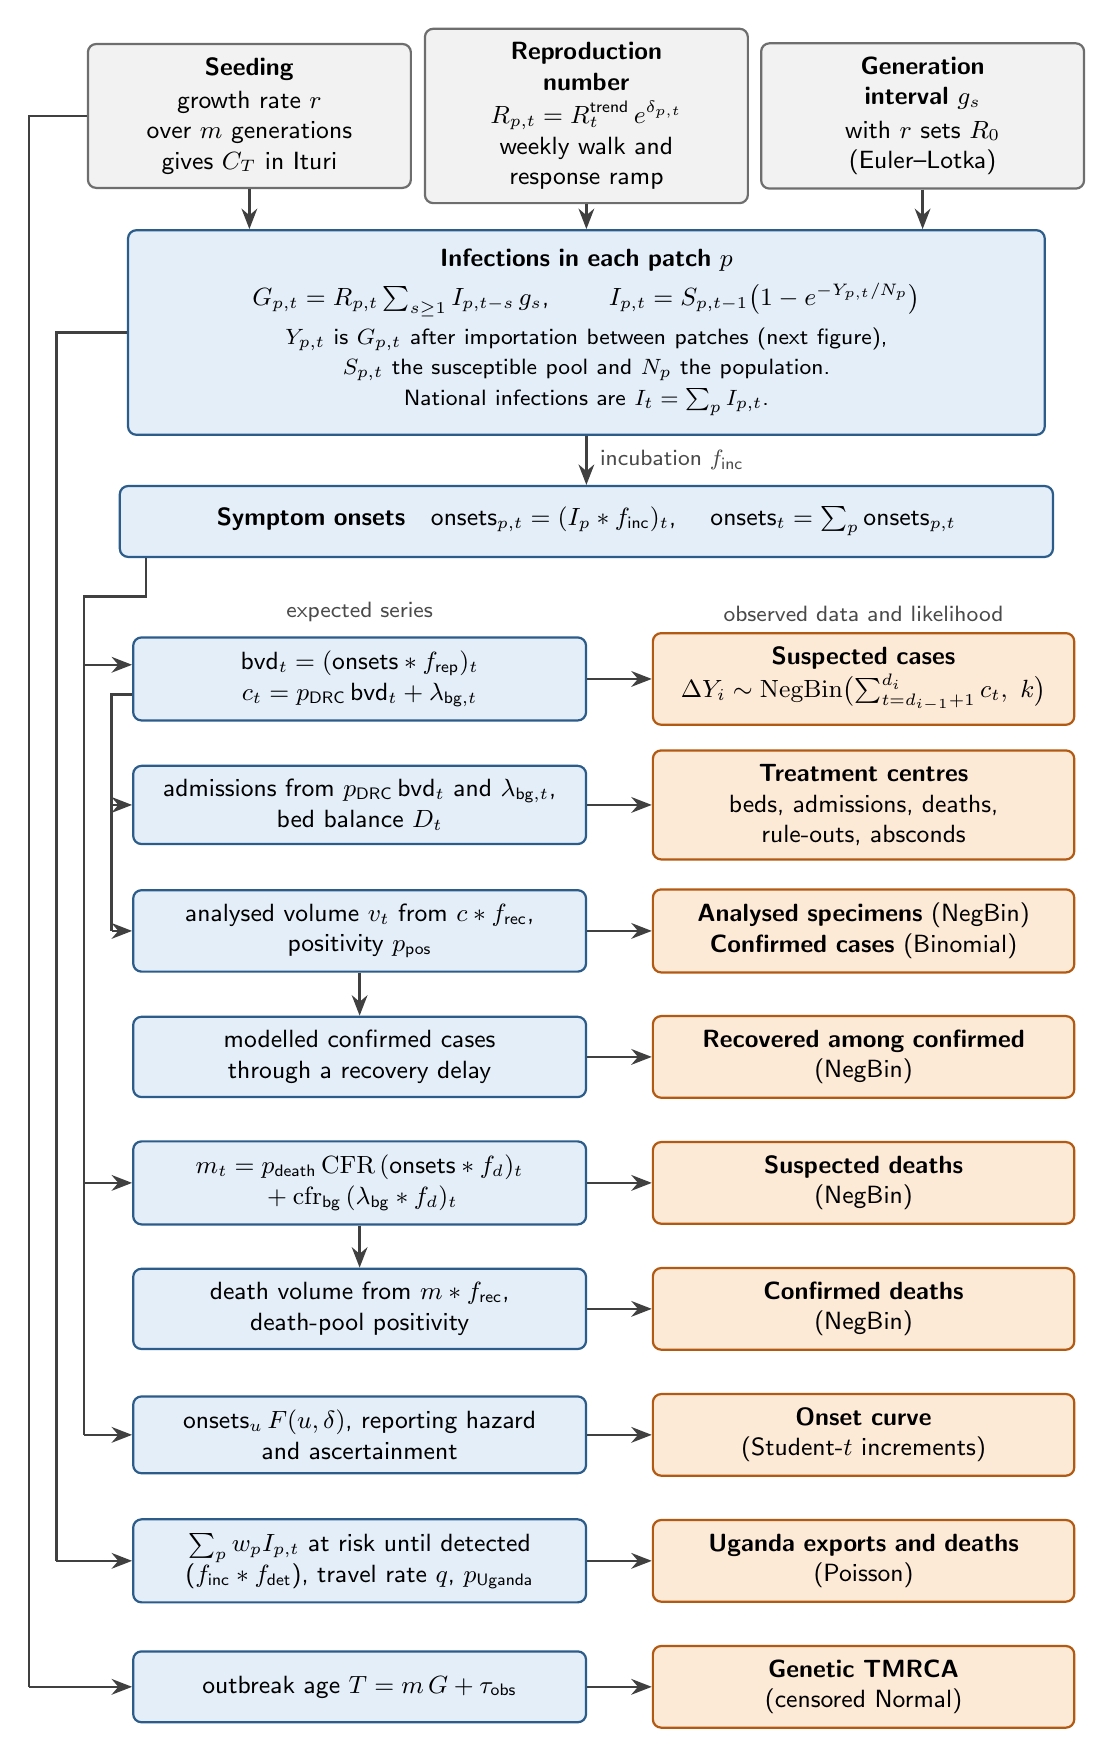
\begin{tikzpicture}[x=1cm,y=1cm]

% Latent column, data column and the left buses.
\def\xl{-2.15}
\def\xr{4.25}
\def\wl{5.4cm}
\def\wr{5.0cm}
\def\bcase{-5.3}  % suspected-case branch bus
\def\bon{-5.65}   % onsets bus
\def\binf{-6.0}   % infections bus
\def\bseed{-6.35} % seeding bus

% ---- Parameters ----------------------------------------------------------
\node[param, text width=3.75cm] (seed) at (-3.55,0)
  {\textbf{Seeding}\\[1pt] growth rate $r$\\ over $m$ generations\\ gives $C_T$ in Ituri};
\node[param, text width=3.75cm] (rt) at (0.73,0)
  {\textbf{Reproduction}\\ \textbf{number}\\[1pt]
   $R_{p,t} = R^{\text{trend}}_t\, e^{\delta_{p,t}}$\\ weekly walk and\\ response ramp};
\node[param, text width=3.75cm] (gi) at (5.0,0)
  {\textbf{Generation}\\ \textbf{interval} $g_s$\\[1pt] with $r$ sets $R_0$\\ (Euler--Lotka)};

% ---- Infections ----------------------------------------------------------
\node[latent, text width=11.15cm, inner sep=7pt] (inf) at (0.73,-2.75)
  {\textbf{Infections in each patch} $p$\\[3pt]
   $G_{p,t} = R_{p,t} \sum_{s \ge 1} I_{p,t-s}\, g_s$, \qquad
   $I_{p,t} = S_{p,t-1}\bigl(1 - e^{-Y_{p,t}/N_p}\bigr)$\\[3pt]
   {\footnotesize $Y_{p,t}$ is $G_{p,t}$ after importation between patches (next figure),}\\
   {\footnotesize $S_{p,t}$ the susceptible pool and $N_p$ the population.}\\
   {\footnotesize National infections are $I_t = \sum_p I_{p,t}$.}};

\foreach \n in {seed,rt,gi}
  \draw[flow] (\n.south) -- (\n.south |- inf.north);

% ---- Onsets --------------------------------------------------------------
\node[latent, text width=11.5cm] (ons) at (0.73,-5.15)
  {\textbf{Symptom onsets}\quad
   $\text{onsets}_{p,t} = (I_{p} * f_{\text{inc}})_t$, \quad
   $\text{onsets}_t = \sum_p \text{onsets}_{p,t}$};
\draw[flow] (0.73,0 |- inf.south) -- (ons.north)
  node[edgelabel, midway, right=3pt] {incubation $f_{\text{inc}}$};

% ---- Streams: latent expectation (left) and data with likelihood (right) --
\def\ya{-7.15}
\def\yb{-8.75}
\def\yc{-10.35}
\def\yd{-11.95}
\def\ye{-13.55}
\def\yf{-15.15}
\def\yg{-16.75}
\def\yh{-18.35}
\def\yi{-19.95}

\node[note, anchor=south] at (\xl,{\ya+0.6}) {expected series};
\node[note, anchor=south] at (\xr,{\ya+0.6}) {observed data and likelihood};

\node[latent, text width=\wl] (rep) at (\xl,\ya)
  {$\text{bvd}_t = (\text{onsets} * f_{\text{rep}})_t$\\
   $c_t = p_{\text{DRC}}\, \text{bvd}_t + \lambda_{\text{bg},t}$};
\node[latent, text width=\wl] (tc) at (\xl,\yb)
  {admissions from $p_{\text{DRC}}\,\text{bvd}_t$ and $\lambda_{\text{bg},t}$,\\
   bed balance $D_t$};
\node[latent, text width=\wl] (lab) at (\xl,\yc)
  {analysed volume $v_t$ from $c * f_{\text{rec}}$,\\ positivity $p_{\text{pos}}$};
\node[latent, text width=\wl] (rec) at (\xl,\yd)
  {modelled confirmed cases\\ through a recovery delay};
\node[latent, text width=\wl] (dth) at (\xl,\ye)
  {$m_t = p_{\text{death}}\,\mathrm{CFR}\,(\text{onsets} * f_d)_t$\\
   ${}+ \mathrm{cfr}_{\text{bg}}\,(\lambda_{\text{bg}} * f_d)_t$};
\node[latent, text width=\wl] (cd) at (\xl,\yf)
  {death volume from $m * f_{\text{rec}}$,\\ death-pool positivity};
\node[latent, text width=\wl] (oc) at (\xl,\yg)
  {$\text{onsets}_u\, F(u, \delta)$, reporting hazard\\ and ascertainment};
\node[latent, text width=\wl] (ex) at (\xl,\yh)
  {$\sum_p w_p I_{p,t}$ at risk until detected\\
   ($f_{\text{inc}} * f_{\text{det}}$), travel rate $q$, $p_{\text{Uganda}}$};
\node[latent, text width=\wl] (age) at (\xl,\yi)
  {outbreak age $T = m\,G + \tau_{\text{obs}}$};

\node[data, text width=\wr] (d_rep) at (\xr,\ya)
  {\textbf{Suspected cases}\\[1pt]
   $\Delta Y_i \sim \mathrm{NegBin}\bigl(\textstyle\sum_{t = d_{i-1}+1}^{d_i} c_t,\ k\bigr)$};
\node[data, text width=\wr] (d_tc) at (\xr,\yb)
  {\textbf{Treatment centres}\\ beds, admissions, deaths,\\ rule-outs, absconds};
\node[data, text width=\wr] (d_lab) at (\xr,\yc)
  {\textbf{Analysed specimens} (NegBin)\\ \textbf{Confirmed cases} (Binomial)};
\node[data, text width=\wr] (d_rec) at (\xr,\yd)
  {\textbf{Recovered among confirmed}\\ (NegBin)};
\node[data, text width=\wr] (d_dth) at (\xr,\ye)
  {\textbf{Suspected deaths}\\ (NegBin)};
\node[data, text width=\wr] (d_cd) at (\xr,\yf)
  {\textbf{Confirmed deaths}\\ (NegBin)};
\node[data, text width=\wr] (d_oc) at (\xr,\yg)
  {\textbf{Onset curve}\\ (Student-$t$ increments)};
\node[data, text width=\wr] (d_ex) at (\xr,\yh)
  {\textbf{Uganda exports and deaths}\\ (Poisson)};
\node[data, text width=\wr] (d_age) at (\xr,\yi)
  {\textbf{Genetic TMRCA}\\ (censored Normal)};

\foreach \a in {rep,tc,lab,rec,dth,cd,oc,ex,age}
  \draw[flow] (\a) -- (d_\a);

% Onsets bus: three streams read straight off the onsets.
\draw[line width=0.9pt, draw=black!75]
  ([xshift=0.35cm]ons.south west) coordinate (o0)
  -- (o0 |- 0,{\ya+1.05}) -| (\bon,\yg);
\draw[flow] ([yshift=0.18cm]rep.west -| \bon,0) -- ([yshift=0.18cm]rep.west);
\draw[flow] (\bon,\ye) -- (dth.west);
\draw[flow] (\bon,\yg) -- (oc.west);

% Suspected-case branch: reports feed the treatment centres and the
% laboratory, and the laboratory feeds the recoveries.
\draw[line width=0.9pt, draw=black!75]
  ([yshift=-0.2cm]rep.west) -- ([yshift=-0.2cm]rep.west -| \bcase,0) -- (\bcase,\yc);
\draw[flow] (\bcase,\yb) -- (tc.west);
\draw[flow] (\bcase,\yc) -- (lab.west);
\draw[flow] (lab) -- (rec);
\draw[flow] (dth) -- (cd);

% Infections bus: the exports read the infections.
\draw[line width=0.9pt, draw=black!75]
  (inf.west) -- (inf.west -| \binf,0) -- (\binf,\yh);
\draw[flow] (\binf,\yh) -- (ex.west);
% Seeding bus: the outbreak age is the cryptic phase plus the window.
\draw[line width=0.9pt, draw=black!75]
  (seed.west) -- (seed.west -| \bseed,0) -- (\bseed,\yi);
\draw[flow] (\bseed,\yi) -- (age.west);

\end{tikzpicture}
\end{document}
